\documentclass{article}
\usepackage[utf8]{inputenc}
\usepackage{graphicx}
\usepackage{float}
\usepackage{listings}
\usepackage{hyperref}
\usepackage{amsmath}


\hypersetup{
    colorlinks=true,
    linkcolor=blue
}

\title{FYS3150 - Computational Physics \\ Project 1}
\author{Philip Hoel}
\date{\today}

\begin{document}

\maketitle

\begin{figure}
    \includegraphics[scale=0.6]{UiO}
\end{figure}

\newpage

\tableofcontents
\newpage

\section{Abstract}
In this project, we will be solving a one dimensional Poisson equation with Dirichlet boundary conditions. The aim is to see the difference in a specialized and general Thomas algorithm for linear sets of equations. We will also see the difference in CPU time between the Thomas algorithm and LU decomposition. We start with some mathematical theory of the problem, then explain the methods used to solve the problem, before we go over to discuss the results and make a conclusion.

\section{Introduction}
We will be tackling Poisson's equation
$$\nabla^{2}\Phi = -4\pi\rho(\mathbf{r})$$
through different numerical algorithms using C++.
We will be focusing on linear algebra. The techniques will be compared with respect to speed and accuracy. \\
For programming, we will have a object oriented angle. And we will be using Python as a scripting language for plotting. All code generated can be found at \href{https://github.com/philhoel/Computational-Physics}{github/Philhoel}.

\newpage
\section{Theory}

\subsection{Stating the project}
As stated in the introduction, this project is calculating Poisson's equation
$$\nabla^{2}\Phi = -4\pi\rho(\mathbf{r})$$
and with spherical symmetry, we can simplify the equation to a one dimensional equation
$$\frac{1}{r^2}\frac{d}{dr}(r^2\frac{d\Phi}{dr}) = -4\pi\rho(r)$$
via the substitution $\Phi (r) = \phi(r)/r$, we can write
$$\frac{d^2 \phi}{dr^2} = -4\pi r\rho(r)$$
by letting $\phi \rightarrow u$ and $r \rightarrow x$ we get the general one-dimensional Poisson's equation
$$-\Ddot{u}(x) = f(x)$$
We will now solve this equation with Dirichlet boundary conditions by using linear algebra.
We have the full equation
$$-\Ddot{u}(x) = f(x) \qquad x \in (0,1) \qquad u(0) = u(1) = 0$$
where we discretized $u$ as $y_i$, with grid points $x_i = i\cdot h$. \\
$x_0 = 0$ and $x_n+1 = 1$, $ h = \frac{1}{n + 1}$. \\
We approximate the second derivative to
$$-\frac{y_{i+1} + y_{i-1} - 2y_i}{h^2} = f_i \qquad for\ i = 1, 2...,n$$
where $f_i = f(x_i)$. By using linear algebra, we can write this as
$$A\mathbf{y} = \mathbf{q}$$
here $A$ is a $n \times n$ tridiagonal matrix and $\mathbf{q} = h^2f_i$.
We have the analytic equation for $u$, which is
$$u(x) = 1 - (1 - e^{-10})x - e^{-10x}$$
if we derive it twice, we'll get
$$f(x) = 100e^{-10x}$$
This will be the analytic function we will compare our numerical solutions to.

\subsection{Setting up linear equation}
If we now multiply with $h^2$ on each side of the discretized equation, we get
$$-y_{i-1} + 2y_i - y_{i+1} = h^2f_i = q_i$$
if we pull out the numbers
\[
[-1\ 2\ -1] \cdot
\begin{bmatrix}
y_{i-1} \\
y_i \\
y_{i+1}
\end{bmatrix}
=
\begin{bmatrix}
q_{i-1} \\
q_{i} \\
q_{i+1}
\end{bmatrix}
\]
Now to make it for all $i$, we recognize that we can't have $y_{i-1}$ in the first one and $y_{i+1}$ at the last one. We then get
\[
\begin{bmatrix}
2 & -1 & 0 & ... & ... & ... \\
-1 & 2 & -1 & ... & ... & ... \\
0 & -1 & 2 & -1 & ... & ... \\
. & ... & ... & ... & ... & ... \\
. & ... & ... & -1 & 2 & -1 \\
. & ... & ... & ... & -1 & 2
\end{bmatrix}
\begin{bmatrix}
y_1 \\
y_2 \\
... \\
... \\
... \\
y_n
\end{bmatrix}
=
\begin{bmatrix}
q_1 \\
q_2 \\
... \\
... \\
... \\
q_n
\end{bmatrix}
\]

\subsection{A general algorithm}
When creating tridiagonal matrix, most of the entries are $0$, and as $n$ grows, we use more and more unnecessary computing power. To get around this, we will put all entries from each diagonal in its own vector. This will give us the equation
\[
\begin{bmatrix}
b_1 & c_1 & 0 & ... & ... & ... \\
a_1 & b_2 & c_2 & ... & ... & ... \\
0 & a_2 & b_3 & c_3 & ... & ... \\
. & ... & ... & ... & ... & ... \\
. & ... & ... & a_{n-2} & b_{n-1} & c_{n-1} \\
. & ... & ... & ... & a_{n-1} & b_{n}
\end{bmatrix}
\begin{bmatrix}
y_1 \\
y_2 \\
... \\
... \\
... \\
y_{n}
\end{bmatrix}
=
\begin{bmatrix}
q_1 \\
q_2 \\
... \\
... \\
... \\
q_{n}
\end{bmatrix}
\]
Here we start with forward substitution and our equations becomes
$$b_i = b_i - \frac{a_i}{b_{i-1}}c_{i-1}$$
$$q_i = q_i - \frac{a_{i-1}}{b_{i-1}}q_{i-1}$$
and then the backward substitution, which starts from the last element
$$y_i = \frac{(q_i - c_i)y_{i+1}}{b_i}$$

\subsection{A special algorithm}
Since we know the elements of the matrix, we can make a special algorithm as well. We know that $b_1 = 2$ and that all $a$ and all of $c$ is $-1$.
$$b_i = 2 - \frac{1}{b_{i-1}} = 2 - \frac{i - 1}{i}$$
We put this into the other equations and get the forward
$$q_i = q_i - \frac{(i - 1}{i}q_{i-1}$$
and the backward substitution
$$y_i = q_i + \frac{y_{i+1}i}{i + 1}$$

\subsection{Method}

\subsubsection{C++}
We write our code in C++. By choosing to solve the problem with an object oriented code, we make enhance the readability and reuseability. We start by defining our vectors. We include the Armadillo library for easy access to linear algebra functionality. In the constructor of the class, we take in $n$ as an parameter and store it as a class variable. Now we can easily make a member function for whatever we need to calculate and we start by defining a function $general\_algorithm()$ and a function $special\_algorithm()$. After this define a few functions for writing the values to a file.

\subsubsection{Python}
Since plotting the results in C++ is more work than necessary, we write the values to a file and make a python script to read and plot the values. The python script takes in 3 files from the command line. One for each different calculation. By making a make file, we can easily compile and run the c++ file and run python as many times as needed by only running the make file.

\newpage
\section{Results}

\subsection{Plots}
From the plots, we see that the general algorithm is pretty accurate from the beginning. The special algorithm is trading it's accuracy for speed, but as $n$ grows, so does the accuracy of the special algorithm as well.

\begin{figure}[H]
    \centering
    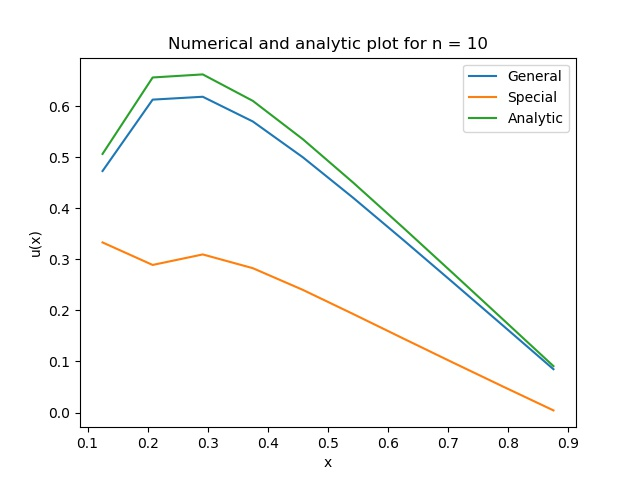
\includegraphics[scale=0.6]{Project1/plot_n_10.jpg}
\end{figure}

\begin{figure}[H]
    \centering
    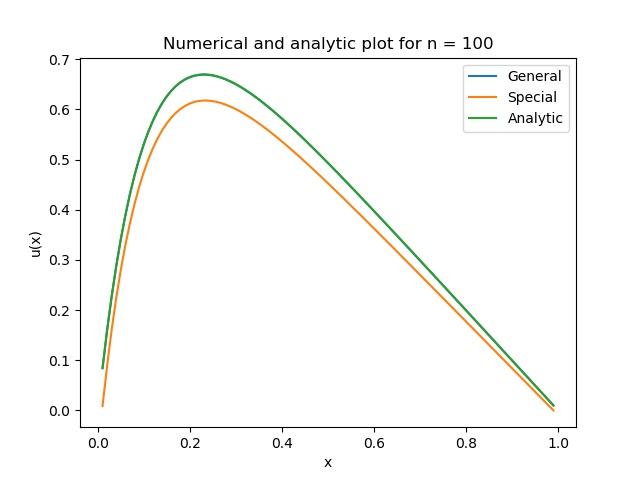
\includegraphics[scale=0.6]{Project1/plot_n_100.jpg}
\end{figure}

\begin{figure}[H]
    \centering
    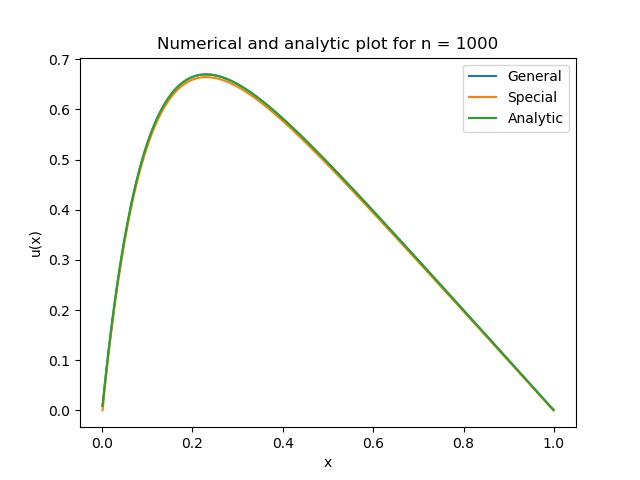
\includegraphics[scale=0.6]{Project1/plot_n_1000.jpg}
\end{figure}

\subsection{Relative errors}

The relative error is calculated by taking the max value of each 
$$\epsilon_i = log_{10}\Big(\Big|\frac{y_i - u_i}{u_i}\Big|\Big)$$

\begin{tabular}{|c|c|}
    \hline
    n & \epsilon \\
    \hline
    10^1 &  -1.1797\\
    10^2 & -3.08804 \\
    10^3 & -5.08005 \\
    10^4 & -7.07929 \\
    10^5 & -8.84297 \\
    10^6 & -6.07551 \\
    10^7 & -5.52523 \\
    \hline
\end{tabular} \\
as we can see from the table, the error is smallest at $n = 10^5$

\subsection{Runtime differences}
We also check the runtime of our algorithm compared to the LU decomposition in Armadillo lib.
\begin{figure}[H]
    \centering
    \includegraphics{Project1/Skjermbilde 2020-09-09 kl. 21.12.09.png}
    \caption{Caption}
    \label{fig:my_label}
\end{figure}
\noindent
as we can see, the difference become drastically different as $n$ increases. This is run up to $n = 10^4$, after that, the matrix got too big and delivered an error message. The CPU time is measured in seconds.

\newpage
\section{Conclusion}
In conclusion, we see that as the number of steps increases, we can greatly benefit from a specialized algorithm. We can also conclude that the Thomas algorithm is much better in both speed and memory than the LU decomposition.

\section{References}
Morten Hjorth-Jensen - Computational Physics: Lecture Notes \\
David C. Lays, Steven R. Lay, Judi J. McDonald - Linear Algebra and it's Applications \\
Wikipedia - Tridiagonal\_matrix

\end{document}